\chapter{Study}
Basic stats here:
we ran over X days
over data points

\section{Reader Demographics}

\section{Media Favorability of Candidates}
Each reader was asked to score the five stories according to how favorable each one was to the featured candidate (by headline). 

\begin{figure}[h!] 
\centering
  \fbox{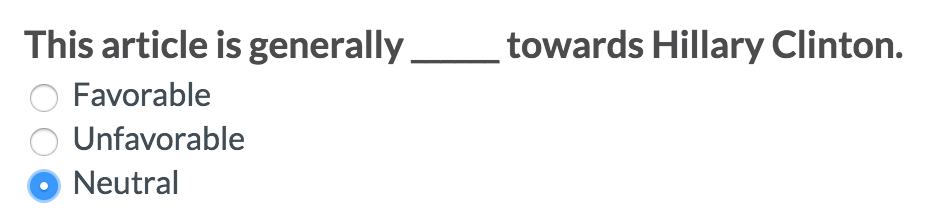
\includegraphics[width=0.5\textwidth]{favorability_question}}
  \caption{Example of favorability scoring question}
\end{figure}
 
Scores were collected on a three-point scale, Favorable (1), Unfavorable (-1), or Neutral (0).

Overall, media coverage of Trump was viewed as most negatively biased, with over half of stories (51.1\%) viewed as unfavorable towards the candidate.

Of the stories shown, both Sanders and Clinton were viewed as having more positive than negative coverage, at 38.9\% of the 180 annotations being positive. Sanders also had the least negative coverage, with only 18.3\% stories shown being viewed as negatively biased against the candidate. Republican candidate Cruz was also seen to have more negative (33.3\%) than positive (28.9\%) stories about him, although the majority were seen as neutral (37.8\%).

\begin{figure}[h!] 
\centering
  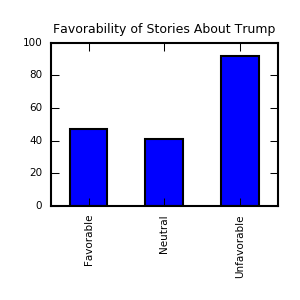
\includegraphics[width=0.45\textwidth]{Trump_favorability} 
  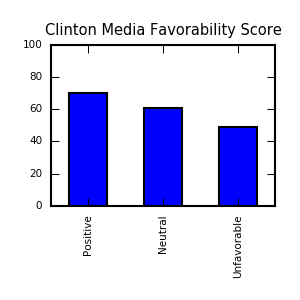
\includegraphics[width=0.45\textwidth]{Clinton_favorability} 
  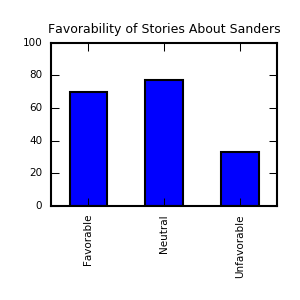
\includegraphics[width=0.45\textwidth]{Sanders_favorability} 
  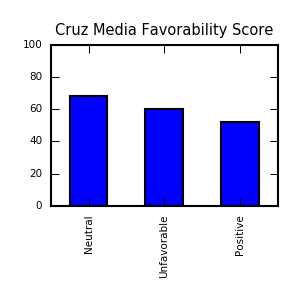
\includegraphics[width=0.45\textwidth]{Cruz_favorability} 
  \caption{Media Favorability of Candidates}
\end{figure}

These trends persist when we filter responses by stories that were considered trustworthy or at least neutral (score > 0).

\begin{figure}[h!] 
\centering
  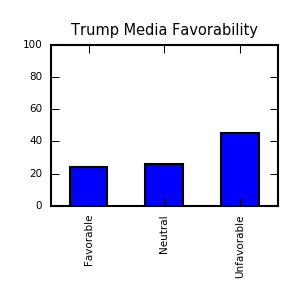
\includegraphics[width=0.45\textwidth]{Trump_favorability_trust_gt_0} 
  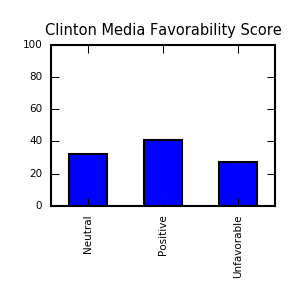
\includegraphics[width=0.45\textwidth]{Clinton_favorability_trust_gt_0} 
  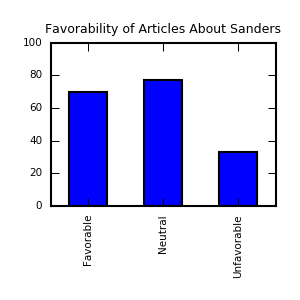
\includegraphics[width=0.45\textwidth]{Sanders_favorability_trust_gt_0} 
  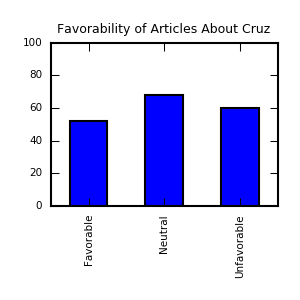
\includegraphics[width=0.45\textwidth]{Cruz_favorability_trust_gt_0} 
  \caption{Media Favorability of Candidates, Trustworthy Articles}
\end{figure}

In the following section, we examine more patterns of media trustworthiness.


\section{Media Trustworthiness}

Each reader was also asked to score the five stories according to how trustworthy they found each to be. 

\begin{figure}[h!] 
\centering
  \fbox{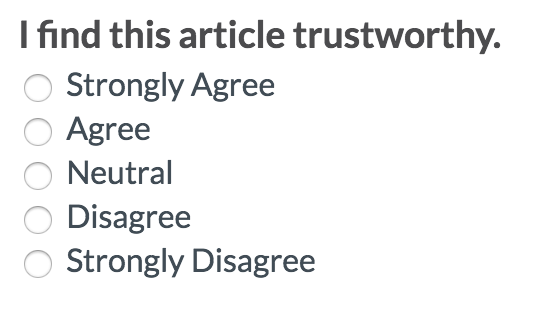
\includegraphics[width=0.35\textwidth]{trustworthy_question}}
  \caption{Example of trustworthiness scoring question}
\end{figure}

Scores were collected on a five-point (Likert) scale: Strongly Agree (2), Agree (1), Neutral (0), Disagree (-1), Strongly Disagree (-2). Overall, readers seldom slected ``Strongly Disagree'', and the option consisted of less than 2\% of all choices.

In the analysis below, we collapse the results into three categories: Agree (> 0), Neutral (0), and Disagree (<0).

Despite reportings on national distrust of news, the majority of stories were marked as trustworthy for all candidates.

\begin{figure}[h!] 
\centering
  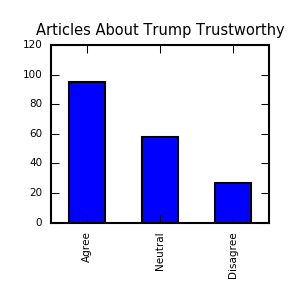
\includegraphics[width=0.45\textwidth]{Trump_trustworthiness_binary} 
  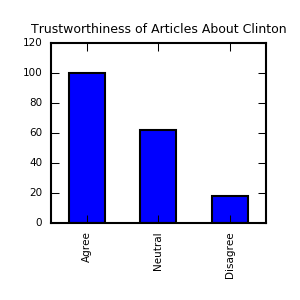
\includegraphics[width=0.45\textwidth]{Clinton_trustworthiness_binary} 
  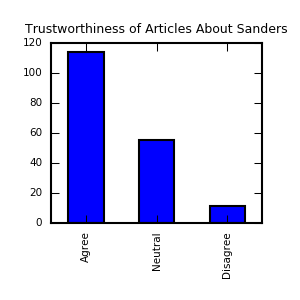
\includegraphics[width=0.45\textwidth]{Sanders_trustworthiness_binary} 
  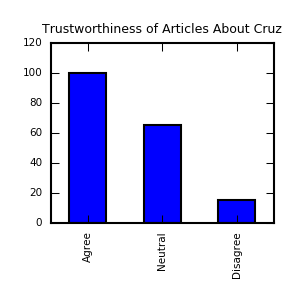
\includegraphics[width=0.45\textwidth]{Cruz_trustworthiness_binary} 
  \caption{Media Trustworthiness of Candidate Coverage}
\end{figure}

 Sanders has strongest trustworthiness, most favorable



 

\section{Overall Bias Reportings}


% This is an example of how you would use tgrind to include an example
% of source code; it is commented out in this template since the code
% example file does not exist.  To use it, you need to remove the '%' on the
% beginning of the line, and insert your own information in the call.
%
%\tagrind[htbp]{code/pmn.s.tex}{Post Multiply Normalization}{opt:pmn}
 